\chapter{Introduction}
What is dark matter? For a question so central to cosmology and particle physics, the prospects for finding an answer do not at first glance seem promising. The interaction of dark matter (DM) particles must be very weak in order to evade a myriad of bounds set by precision astrophysical and cosmological tests. Our failure to observe dark matter particles thus far tells us that their interactions must be even weaker still. The effort to detect these interactions both on Earth and in the wider universe is a vast technological and scientific challenge.

However, such efforts are advancing rapidly. The detection of particle DM using terrestrial detectors would give strong clues about the nature and identity of DM. However, the analysis of these so-called `direct detection' experiments is plagued with uncertainties. One such uncertainty is in our understanding of the astrophysical speed distribution of dark matter, which influences the typical energies which would be deposited in a detector in the lab. If these uncertainties can be overcome, direct detection promises to be a powerful probe of both the particle physics and astrophysics of DM.

Without a detection of a possible particle candidate, then, the question `What is dark matter?' is perhaps best answered by reviewing the current evidence for its existence. Evidence for dark matter is found on scales from the Milky Way up to the cosmological horizon, with a range of observations which cannot be adequately explained with the observed constituents of the universe. Dark matter is an invisible component introduced to reconcile these observations with the known laws of physics - most importantly, General Relativity. Beyond this general definition, there are a wide range of particle physics candidates which may play the role of dark matter. These typically derive from theories of physics beyond the Standard Model, meaning that the study of the properties of dark matter can shed light on theories of high energy physics. Many of these proposed dark matter candidates have weak but non-zero interactions with particles of the Standard Model, leading to several avenues through which it is hoped the non-gravitational detection of dark matter may soon be achieved.

In this chapter, we summarise the evidence in support of the dark matter paradigm, including constraints from precision cosmology. We discuss some of the features which particle DM must possess, as well as describing a few specific candidates in more detail. Finally, we discuss current progress and constraints from direct and indirect searches for particle dark matter.

\section{Evidence for dark matter}

\note{Definitely need to add more in the dark matter evidence section!}

Dark matter is a key component of the \LCDM paradigm of modern cosmology. In this framework, the energy density of the universe today is dominated by the constant and uniform contribution of the vacuum, $\Lambda$. This contribution exerts a negative pressure and drives the accelerating expansion of the universe which was the subject of the 2011 Nobel Prize in Physics \cite{Riess:1998, Perlmutter:1999}. However, the formation of structure in the early universe is driven by the clustering of a non-interacting, slow moving and as yet undetected matter component \cite{Kolb:1990}, Cold Dark Matter (CDM). The fact that DM is non-interacting (or at least, interacts only very weakly) means that it begins to collapse gravitationally earlier in cosmic time than baryonic matter. After decoupling, baryons then fall into the gravitational wells produced by the infalling DM structures. Without DM, the baryonic matter in the universe could not have had enough time to collapse to form the range of gravitationally bound structures we see today \cite{Blumental:1984,Kolb:1990}

Cosmological experiments sensitive to the expansion and structure formation history of the universe allow us to precisely determine the contributions of the various different components to the energy density of the universe (see e.\ g.\  WMAP \cite{Hinshaw:2013}, BOOMERanG \cite{MacTavish:2005}, BOSS \cite{Dawson:2013}, BICEP2 \cite{Ade:2014} and CFHTLenS \cite{Kitching:2014, Fu:2014} to name just a few). For example, Baryon Acoustic Oscillations (BAOs) are a feature imprinted on the distribution of matter in the universe by acoustic waves prior to recombination. BAOs can be measured by using galaxy redshift surveys (such as SDSS \cite{York:2000}) to map out the large scale structure of the universe and they provide a `standard ruler' for measuring cosmological distances. Type-Ia Supernovae provide `standard candles' which can be used to measure luminosity distances in the universe. Redshift surveys of these supernovae \cite{Suzuki:2011} then allow us to reconstruct these distance scales over cosmic time. Complementary information from these probes and others allow us to constrain the expansion history of the universe and therefore the various contributions to the density of the universe.

%Weak lensing surveys can also be used to map the distribution of matter in the universe, but these map the distribution of all matter, not only that of visible galaxies.

%Red shift space distortions \cite{Peacock:2001}
%Measuring the correlations of galaxies and fitting to data \cite{Percival:2001}

\note{Maybe need a paragraph on early stuff (CMB) and a paragraph on late stuff (BAOs and RSD)}

A particularly sensitive probe for determining the dark matter contribution to the energy budget of the universe is the measurement of the temperature anisotropies of Cosmic Microwave Background (CMB) photons. These contain an imprint of the acoustic oscillations of the baryon-photon fluid during the era of recombination. The scale of these oscillations is sensitive to the size of the gravitational potential generated in the early universe by dark matter, which does not interact with the photons \cite{Kolb:1990}. The recent Planck experiment \cite{PlanckI:2013} measured the angular power spectrum of these CMB temperature anisotropies. Figure~\ref{fig:intro:CMB} shows the results of these measurements, as well as the best fit 6-parameter \LCDM model. The contributions of the cosmological constant, the total matter component, and the separate baryonic and dark matter components to the total energy density of the universe are shown in Table~\ref{tab:intro:Planck}, constrained with an accuracy of less than 3\%. These results point to the conclusion that $\sim$84\% of the matter content of the universe is in fact dark.

%\todo{Read for details: arXiv:1404.5415}


\begin{figure}[h]

  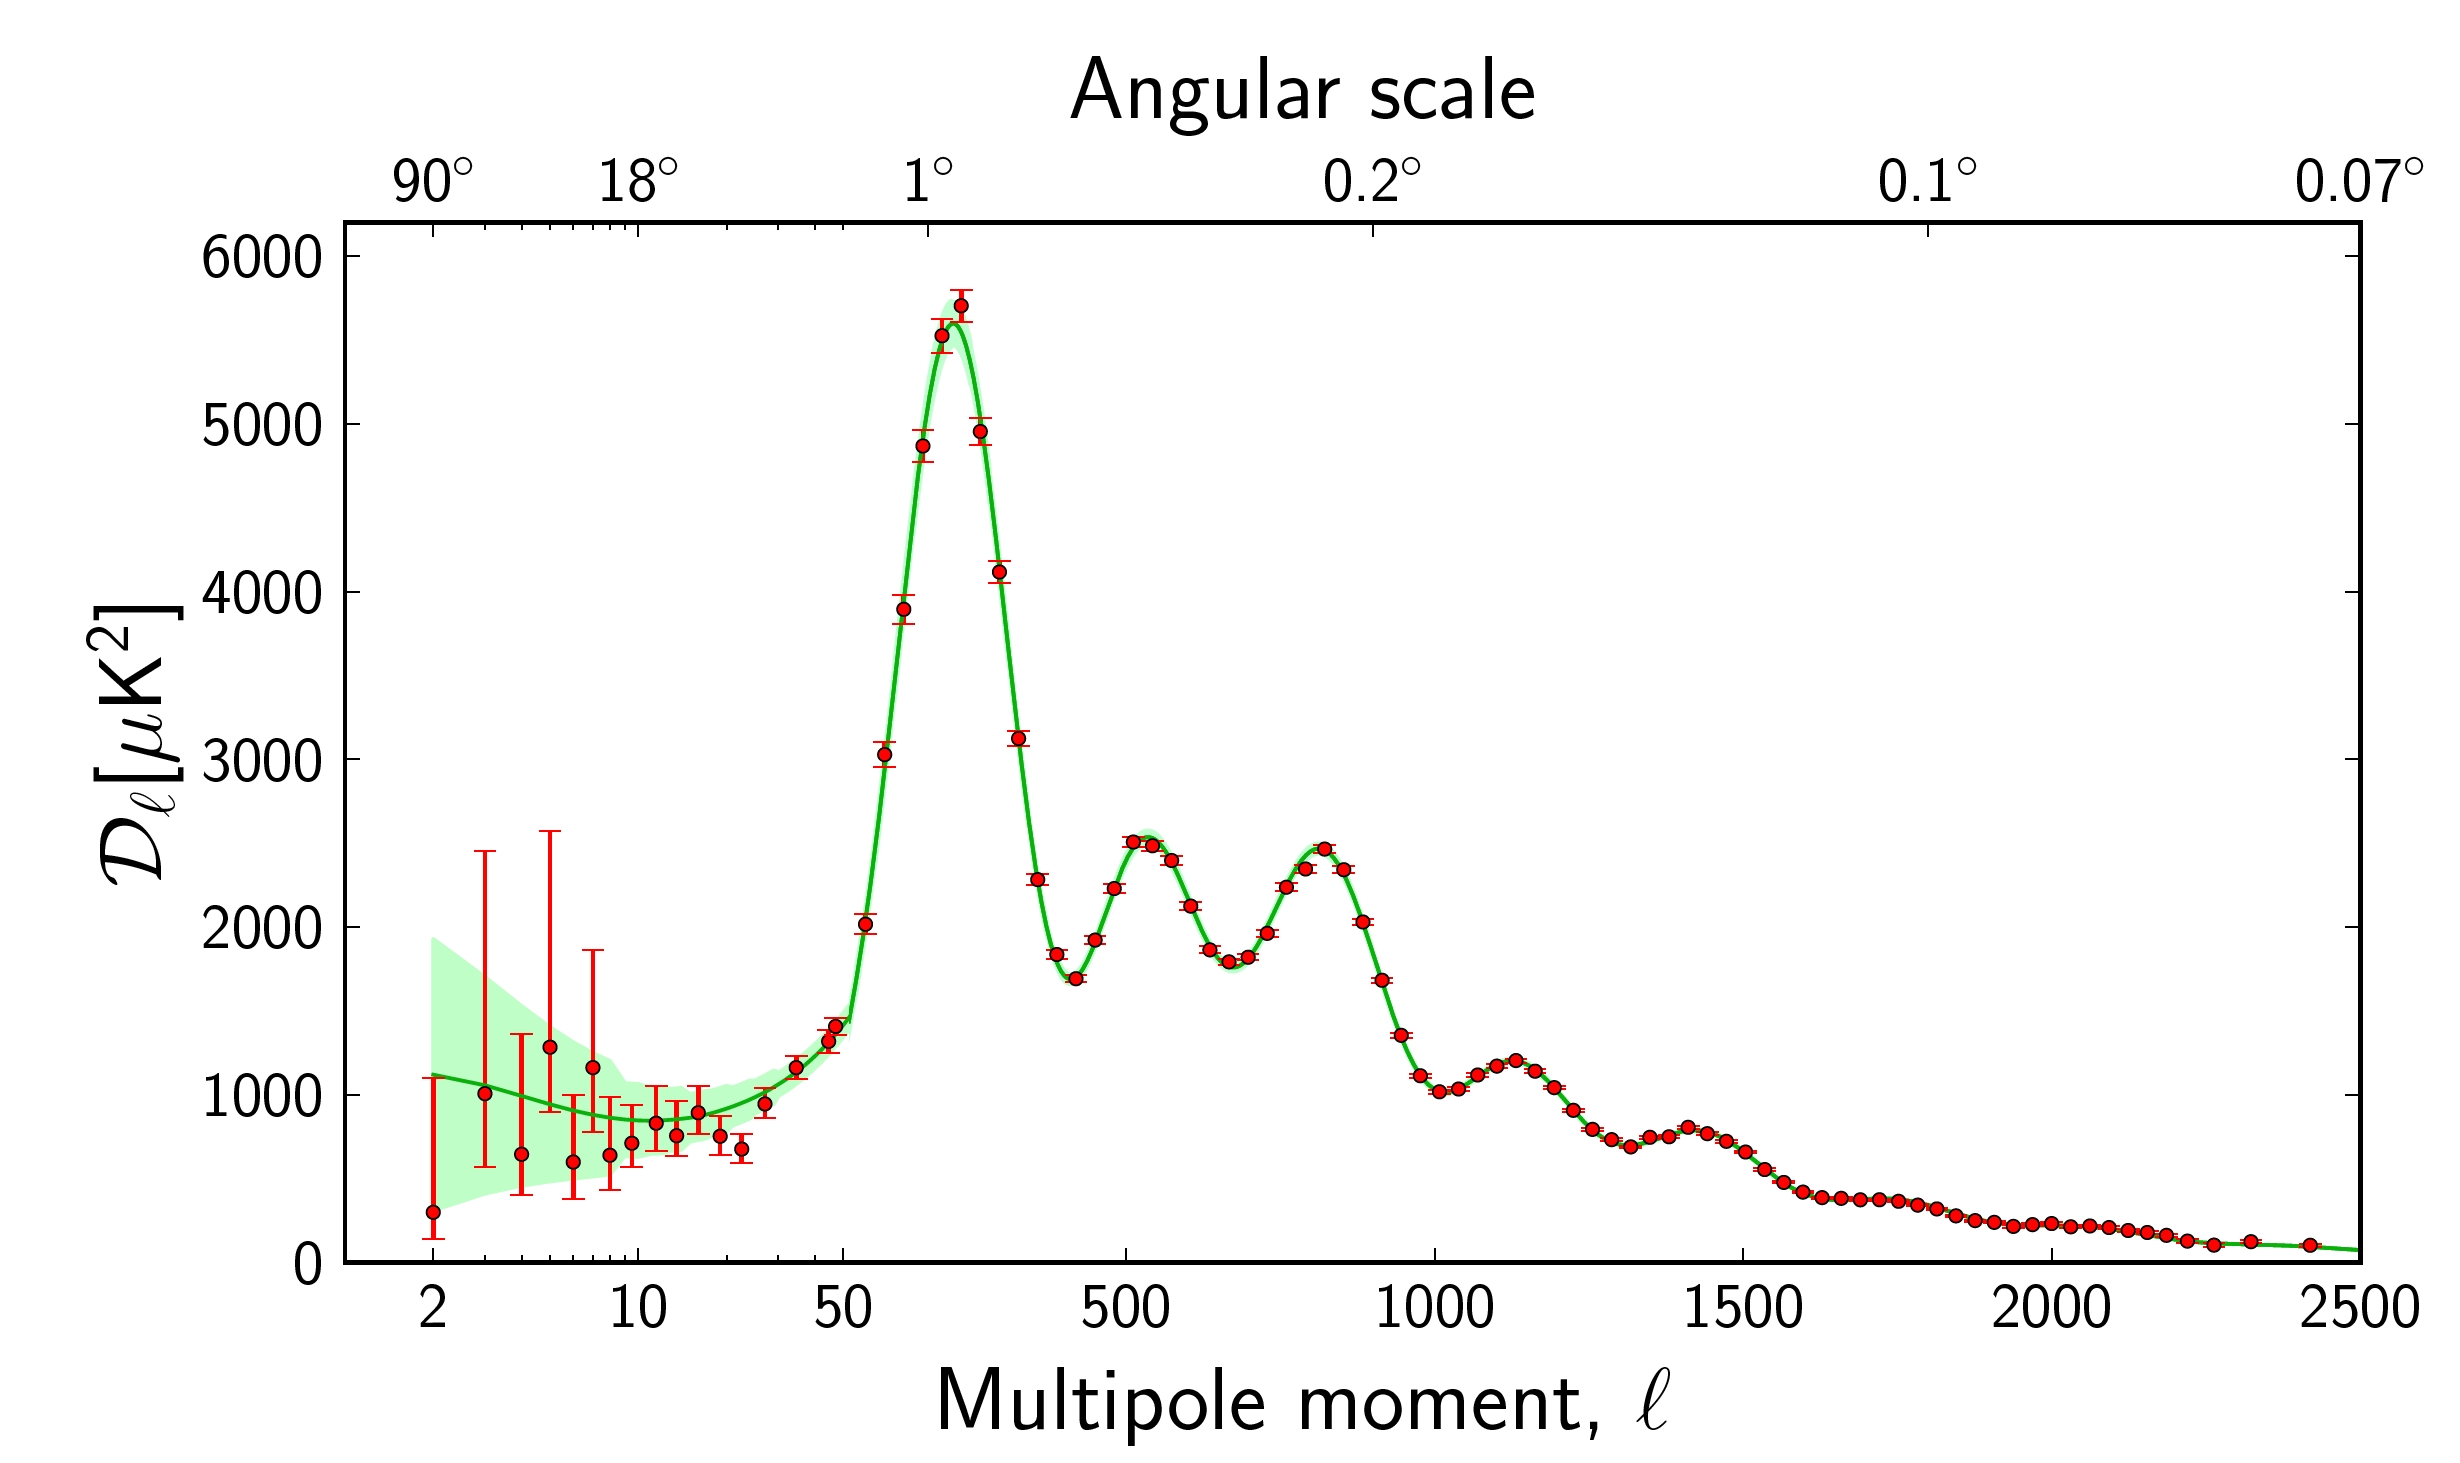
\includegraphics[width=\textwidth]{CMBanisotropies.jpg}
  \caption[CMB anisotropies measured by the Planck experiment]{Angular power spectrum of CMB temperature anisotropies as a measured bythe Planck satellite. Data are shown as red points with the best fit \LCDM cosmological model shown as a green line. Reproduced from Ref.~\cite{PlanckI:2013}.}
  \label{fig:intro:CMB}
\end{figure}


\begin{table}

  \begin{center}
	\begin{tabular}{cc}
        \hline\hline
        Parameter & 68\% limits \\
        \hline
        $\Omega_\Lambda$ & 0.686 $\pm$ 0.020 \\
        $\Omega_m h^2$ & 0.1423 $\pm$ 0.0029 \\
        $\Omega_b h^2$ & 0.02207 $\pm$ 0.00033 \\
        $\Omega_c h^2$ & 0.1196 $\pm$ 0.0031 \\
        \hline\hline
	\end{tabular}
  \end{center}
  \caption[Cosmological parameters obtained by the Planck Collaboration]{Energy density $\Omega$ of the cosmological constant ($\Lambda$), total matter ($m$), and separate baryonic ($b$) and cold dark matter ($c$) components in units of the critical density, as obtained by the Planck Collaboration \cite{PlanckXVI:2013}. The Hubble parameter is defined as $H_0 = 100 \,\,h \, \textrm{km s}^{-1} \textrm{Mpc}^{-1}$.}
  \label{tab:intro:Planck}
\end{table}

However, the evidence for dark matter is not purely cosmological. In 1933, Zwicky measured the velocity dispersion of galaxies in the Coma cluster \cite{Zwicky:1933}. An application of the Virial Theorem indicated a gravitational mass in the cluster which was several hundred times bigger than that expected from the luminosity of the member galaxies. It is now known that some of this mass is in the form of hot ($\sim$1 million K), X-ray emitting intracluster gas \cite{Sanders:2013}. Nonetheless, a discrepancy remains; current estimates of the mass-to-light ratio of the Coma cluster give a value of roughly 150 times that of the Sun \cite{Fusco-Femiano:1994,Makino:1994}. The Coma cluster does not appear to be unusual. Measurements of the masses of a large number of galaxy clusters using gravitational lensing \cite{Okabe:2013}, X-ray observations \cite{Ettori:2013} and dynamical estimates \cite{Carlberg:1995} indicate that a significant fraction of a cluster's mass must be dark.

The success of the \LCDM paradigm is also borne out in results from N-body simulations. These simulations track the evolution of structure in the universe by modeling the dynamics and gravitational interactions of a large number of particles starting from some initial conditions. These may be cosmological simulations, tracing the collapse of the initial density perturbations after decoupling (such as the the Millenium simulation \cite{Springel:2005}), or galaxy-scale simulations, tracing the formation and growth of a small number of galaxies starting from initial conditions at intermediate redshift (such as the Via Lactea \cite{Diemand:2006} and Aquarius \cite{Springel:2008} simulations).

Many N-body simulations are DM-only, simulating only the gravitational dynamics of collisionless particles. However, an increasing number are incorporating baryonic physics such as gas dynamics, as well as stellar evolution, chemical enrichment and a variety of feedback processes (see e.g.~\cite{Mollitor:2014,Vogelsberger:2014}). Appropriately accounting for these factors is extremely complex and in some cases the strength of these processes is unknown and must be tuned in the simulations to match observations \cite{Vogelsberger:2013}. Due in part to these difficulties, the impact of baryonic physics on the formation of galaxies and the properties of DM haloes is still uncertain (see for example Refs.~\cite{Martizzi:2012,Pillepich:2014}). I will revisit this topic - and its consequences for the direct detection of dark matter - in Chapter~\ref{ch:DD}.

A variety of sophisticated computational techniques (such as smoothed particle hydrodynamics \cite{Stinson:2010}, adaptive mesh refinement \cite{Norman:1999} and moving mesh cosmology \cite{Springel:2010}) have been employed and refined to make such simulations computationally feasible and to allow higher and higher resolutions to be reached. In spite of this, computational limitations mean that the highest resolution simulations still use `particle' masses of the order of $10^5 M_{\odot}$ \cite{Pillepich:2014}, many orders of magnitude more massive than the $O$(GeV-TeV) particles expected to make up the universe's dark matter.

In spite of this, a consistent picture has emerged from a vast array of N-body simulations. The distribution of galaxies observed in large scale structure surveys matches that predicted by N-body simulations over a range of distance scales \cite{Springel:2005}. In addition, N-body simulations have begun to accurately reproduce the observed populations of elliptical and spiral galaxies \cite{Vogelsberger:2014}, as well as obtaining Milky Way-like simulated galaxies \cite{Mollitor:2014}. This ability of simulations containing DM to reproduce structures observed in the Universe is further evidence in support of the DM paradigm. Such is the accuracy of N-body simulations that they can be used to generate mock galaxy catalogues which allow statistical and systematic errors to be assessed in real galaxy surveys \cite{Lemson:2006}.



Further evidence for dark matter comes from observations of the rotation curves of spiral galaxies. In particular, the circular velocity of stars in these galaxies is observed to be approximately constant out to large galactocentric distances \cite{Begeman:1991,Persic:1996}. In fact, observations of hydrogen 21cm emission indicate that the constancy of the circular velocity extends well beyond the optical edge of galaxies \cite{Bosma:1981a, Bosma:1981b}.

This is shown schematically in Fig.~\ref{fig:intro:RotationCurves}. The majority of the mass of the luminous disc is concentrated at small radii, suggesting that there should be a Keplerian decay of the circular velocity at large radii: $v \sim r^{-1/2}$. However, the inclusion of an approximately spherically symmetric, non-luminous dark matter halo can reconcile this expectation with the observed flat rotation curves. The density profiles $\rho(r)$ required to provide a good fit to rotation curve data may be consistent with those obtained from N-body simulations, such as the Navarro-Frenk-White profile

\begin{equation}
\label{eq:intro:NFW}
\rho(r) = \frac{\rho_0}{r/R_s(1 + r/R_s)^2}\,,
\end{equation}
which is described by a characteristic density $\rho_0$ and scale radius $R_s$. However, as we discuss in Sec.~ref{sec:intro:problems}, better fits may be obtained by so-called `cored' density profiles. The rotation curve of the Milky Way itself has also been studied \cite{Deason:2012,Lopez-Corredoira:2014,Bhattacharjee:2014} and found to be almost flat. Using a variety of techniques, it is also possible to measure a non-zero DM density near the Sun's position. An understanding of this density has significant implications for the study of dark matter detection and we defer a detailed discussion to Chapter~\ref{ch:DD}.

\begin{figure}[h]

  \centering
  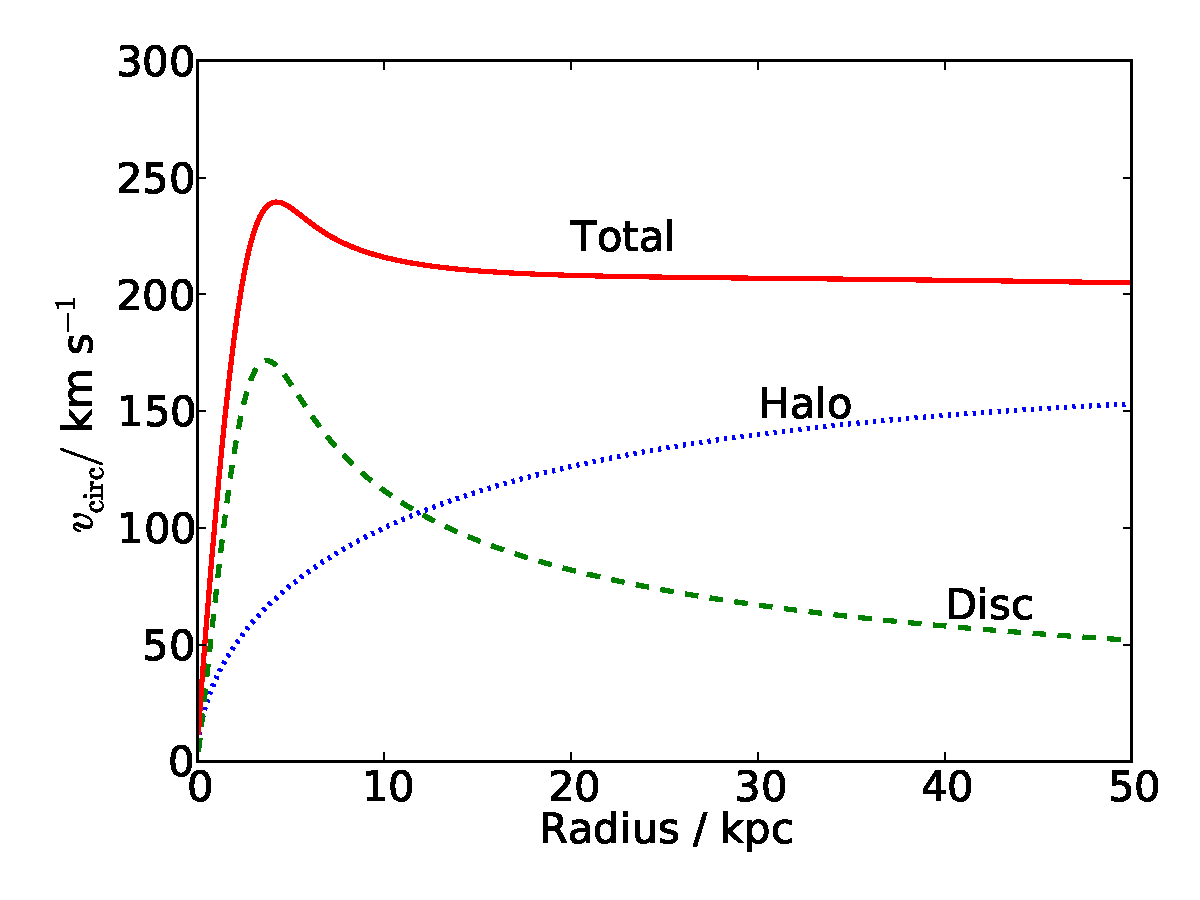
\includegraphics[width=0.8\textwidth]{RotationCurve.pdf}
  \caption[Schematic illustration of galaxy rotation curves]{Schematic illustration of galaxy rotation curves (circular velocity as a function of galactocentric distance). The contribution to the circular velocity from the luminous disc (green dashed line) and dark matter halo (red dotted line) are shown, as well as the total circular velocity (solid blue line). }
  \label{fig:intro:RotationCurves}
\end{figure}

We see that evidence for dark matter appears over a wide range of distance scales, from the cosmological horizon down to our own Milky Way. Dark matter is required to explain the formation and growth of large scale structure, the dynamics of both galaxies and galaxy clusters and the anisotropic temperature distribution of the CMB among others. In spite of this, there remain several problems and unanswered questions with the dark matter paradigm.


\subsection{Problems with dark matter}
\label{sec:intro:problems}
There have emerged several issues with the dark matter dominated model of structure formation as studied with N-body simulations. For example, DM-only simulations predict the existence of a large number of massive subhalos around Milky Way-size galaxies \cite{Springel:2008}. Using semi-analytical models of galaxy formation Kauffmann \etal \cite{Kauffmann:1993} predicted that a Milky Way-size halo should host over 100 subhalos massive enough to support observable satellite galaxies.  However, the known population of dwarf spheroidal (dSph) satellite galaxies for the Milky Way is on the order of 20 \cite{Walker:2009}, although more ultra-faint satellites are still being discovered (e.g. see Ref.~\cite{Belokurov:2010}). This discrepancy between the predicted and observed amount of substructure in CDM structure formation is often referred to as the `missing satellite problem' \cite{Klypin:1999}.

A related issue is the so-called `too big to fail' problem, which concerns the density of dark matter subhalos. In particular, it is found that the most massive DM subhalos found in N-body simulations are too massive to host the brightest of the Milky Way's dSph satellites \cite{Boylan-Kolchin:2011}. If the observed dSph galaxies are hosted instead by less massive subhalos, this leaves a large number of more massive DM halos which have not yet been accounted for \cite{Garrison-Kimmel:2014}.

Finally, there is also a discrepancy between observed and simulated density profiles for dSphs: the `Core-Cusp' problem (for a review, see Ref.~\cite{deBlok:2009}). Cosmological simulations indicate that the DM density should be sharply peaked near the centre of low surface brightness and dSph galaxies \cite{Dubinski:1991, Navarro:1996}. In contrast, observations of the rotation curves of a large number of galaxies suggests the presence of a core - a flat dark matter density profile near the centre \cite{Salucci:2001, Donato:2004}. While these results are still under contention (for example, Ref.~\cite{Hayashi:2004} find rotation curves consistent with \textit{cuspy} density profiles), they may indicate a discrepancy between the process of structure formation in the universe and that implied by \LCDM.

A number of possible solutions to these issues have been suggested. Baryonic effects such as dynamical friction and stellar and supernova feedback (see for example Refs.~\cite{Gritschneder:2013, Amorisco:2014,DelPopolo:2014}) can lead to the expulsion of DM from the centres of subhalos, reducing the total halo mass and leading to a flatter central density profile. Others have suggested that a \textit{warm} dark matter model may be a better fit to the data \cite{Moore:1999, Bode:2001, Maccio:2010}, reducing the amount of structure on small scales, as we will discuss in Sec.~\ref{intro:sec:properties}. Whatever the ultimate resolution of these problems, it is clear that dark matter dominated structures such as dSph galaxies are a testing ground for an even more precise understanding of structure formation in the DM paradigm.

There remains one problem which is of a much more theoretical nature. Dark matter is invoked to account for missing mass in a wide range of scenarios. However, this missing mass has not yet been observed indicating that it must interact only very weakly with photons and other particles of the standard model. In fact, as we shall see, there is strong evidence that particles making up the universe's dark matter cannot be baryonic and must originate from beyond the Standard Model of particle physics. In the next section, we investigate what more can be inferred about the nature of particle dark matter and explore some well-motivated candidates.

\todo{MACHOs? MOND?}

\note{Need consistency between `DM' and `dark matter'}

\section{Alternatives to dark matter}

We have discussed a wide range of evidence for the existence of DM, as well as some unresolved problems with the \LCDM paradigm. Here, we consider the possibility that these observations can be explained not by a new matter species but by a modification to gravity. Milgrom \cite{Milgrom:1983a, Milgrom:1983b, Milgrom:1983c} proposed the idea of Modified Newtonian Dynamics (MOND): for accelerations smaller than some characteristic value $a_0$ the usual Newtonian dynamics no longer holds. In particular, for an acceleration $\mathbf{a}$ in a gravitational field $\Phi_N$, these new dynamics can be written
\begin{equation}
\label{eq:intro:MOND}
\tilde{\mu}(|\mathbf{a}|/a_0)\mathbf{a} = -\nabla \Phi_N\,.
\end{equation}
The interpolation function $\tilde{\mu}$ tends to unity for large values (the Newtonian limit) but tends to $|\mathbf{a}|/a_0$ for values $|\mathbf{a}| \ll a_0$ (the MOND limit).

At large distances fromm the centres of galaxies, the acceleration will drop below $a_0$ and Eq.~\ref{eq:intro:MOND} reduces to $a = v_c(r)^2/r = \sqrt{a_0 \nabla \Phi_N}$, where $v_c$ is the circular velocity. Assuming that there is no dark matter content, the mass $M$ enclosed within a radius $r$ becomes constant and we obtain $|\nabla \Phi_N| \approx GM/r^2$. Combining these, we see that

\begin{equation}
\label{eq:intro:TullyFisher}
v_c(r)^4 \approx GM a_o\,,
\end{equation}
independent of radius. Thus, a flat rotation curve is obtained without the need to invoke DM. Moreover, Eq.~\ref{eq:intro:TullyFisher} is the baryonic Tully-Fisher law, which relates the baryonic mass of a galaxy with the asymptotic rotation velocity. The value for the characteristic acceleration obtained from fits to over 100 galaxies is $a_0 = 1.2 \times 10^{-10} \textrm{ m s}^{-2}$ \cite{Begeman:1991}, which also reproduces the measured proportionality constant in the Tully-Fisher law \cite{McGaugh:2005}.

The phenomological approach of MOND can be recast into a fully covariant theory of modified gravity, known as tensor-vector-scalar (TeVeS) gravity \cite{Bekenstein:2005}. This theory contains new dynamical vector and scalar degrees of freedom and contains a free function, analogous to the interpolation function $\tilde{\mu}$. The formalism for both lensing \cite{Chiu:2005} and cosmological perturbations \cite{Skordis:2006} have both been studied in TeVeS, with perturbations in the new scalar field allowing structure to form without the need for DM.

How then does MOND compare to DM?

\cite{Zhao:2006} Lensing stuff...

MOND requires hot dark matter...

\note{Galaxy cluster discrepancies...}

http://arxiv.org/abs/astro-ph/0508048
http://arxiv.org/abs/astro-ph/0505519
http://arxiv.org/abs/astro-ph/0608602
http://arxiv.org/abs/1002.0849


\section{Properties of dark matter}
\label{intro:sec:properties}

Beyond its gravitational contribution to the universe, we appear to know little about the nature of particle dark matter. However, the success of modern cosmology and the lack of a confirmed detection so far means that we do have a grasp on some of the properties of any potential candidate.

For example, DM can have no significant electromagnetic charge, otherwise it would have been seen in a range of searches \cite{Kudo:2001,Perl:2001,Gninenko:2007,Melchiorri:2007}. DM carrying bare color charge can also be excluded due to the disruption it would cause to galaxy formation \cite{Natarajan:2002} and the formation of the CMB \cite{Chen:2002}. Any particle candidate must also be long-lived - otherwise it cannot play the role of dark matter today. For models in which DM is not indefinitely stable, this allows us to place stringent limits on the lifetime of the DM particle \cite{Amigo:2009,Bell:2010}. %\note{These don't actually come from those arguments, but K.}

In an effort to summarise what is known about dark matter, Taoso \etal \cite{Taoso:2008} present a `10-point test' which must be passed by any particle before it can be considered as a viable dark matter candidate. Here, I will briefly discuss three of these points, namely, that the DM candidate must be cold, produced with the appropriate relic density and compatible with primordial nucleosynthesis.

\subsection{Coldness}

Dark matter cannot be hot. That is, DM must have been travelling non-relativistically when it decoupled from the thermal bath in the early universe. The typical speed of DM particles in the early universe defines the so-called \textit{free-streaming length}. Below this length-scale, density perturbations are suppressed due to Landau damping \cite{Bond:1983}. For non-relativistic species, this free-streaming length scales as $m_\chi^{-1/2}$ for thermal relics of mass $m_\chi$ \cite{Boyanovsky:2008} For particle candidates which are too light - and which therefore travel too quickly after decoupling - small scale structures cannot form and cannot match the distribution of structures we see today. In practise, this typically means that DM cannot have a mass greater than around 1 keV \cite{Narayanan:2000}. It is typically assumed that dark matter is significantly heavier than this, decoupling ultra-non-relativistically in the early universe, rendering it cold.  \textit{Warm} dark matter candidates with keV-scale masses have been suggested to explain the subhalo structures at the scale of dSph galaxies (as has already been discussed). However, \textit{hot} dark matter, which decouples at relativistic speeds, is strongly-constrained and cannot make up more than around 1\% of the total dark matter component \cite{Abazajian:2005, dePutter:2012}.


\begin{comment}
\subsection{Neutrality}

\todo{Condense this into a couple of sentences in the section intro...}

The possibility that charged massive particles (CHAMPs) may account for dark matter was proposed by De Rujula \etal \cite{DeRujula:1990}. Such particles be free and stable or may instead bind with electrons or positrons to form heavy neutral hydrogen-like objects. However, null searches for anomalous hydrogen in sea water \cite{Kudo:2001} and anomalous heavy elements \cite{Hemmick:1990}, as well as searches for CHAMPs in cosmic ray experiments \cite{Perl:2001} indicate that CHAMPs must be present in negligible densities in the Milky Way for masses in the range $10-10^8$ GeV. Millichared DM is also strongly constrained. Searches for neutrino magnetic moments in reactor experiments exclude DM with charge greater than $10^{-5} e$ for keV-scale masses and below \cite{Gninenko:2007}. Searches for distortions in the CMB caused by the interactions of millicharged particles limit the DM charge to be less than $10^{-7} e$ for masses of 1 eV and below \cite{Melchiorri:2007}.

Could DM particles carry a colour charge? In this case, DM particles would interact strongly with particles of the SM. Such strong interactions may disrupt galaxy formation \cite{Natarajan:2002}, distort the CMB due to scattering off baryons \cite{Chen:2002} and have been strongly constrained by experimental searches with the X-ray Quantum Calorimeter \cite{Erickcek:2007} and direct detection experiments \cite{Albuquerque:2004}. %\note{What about weak hypercharge?}

We are left with the conclusion that (without a mechanism for evading the above constraints \cite{AnExample}) DM particles must carry no (or almost no) conventional electromagnetic, weak or strong charge. This rules out all SM particles as accounting for DM hinting strongly that these particles must derive from theories of physics beyond the Standard Model.

%\note{What about current constraints on `dark atoms'?}
\end{comment}
\subsection{Relic density}

In order to account for the dark matter in the universe, a good candidate must be produced in the early universe with sufficient abundance to match the currently observed value $\Omega_c h^2 = 0.1196 \pm 0.0031$ (see Table~\ref{tab:intro:Planck}). If produced with a smaller abundance, the candidate cannot account for the entirety of the universe's dark matter (though it could still contribute, along with other candidates, as in Ref.~\cite{Feldman:2010}). If on the other hand, it is produced with too great an abundance, it could threaten to exceed the DM density constraint set by Planck and overclose the universe.

The standard scenario for the production of dark matter is referred to as thermal freeze-out \cite{Kolb:1990}. In this scenario, DM particles remain in kinetic and chemical equilibrium with SM particles in the very early universe by scattering and annihilation processes. Their number density $n$ follows a Maxwell-Boltzmann distribution

\begin{equation}
n \sim (m/T)^{3/2} \exp(-m/T)\,,
\end{equation}
for a mass $m$ and temperature $T$. As the universe expands, however, the particles become diluted, reducing the interaction rate until eventually the DM particles become decoupled from the SM particles and are `frozen-out.' They are then left with the abundance they had when they decoupled, which is further diluted by the expansion of the universe to become the abundance we see today. The exact relic abundance depends on $\langle \sigma_\mathrm{ann} v\rangle$, the average annihilation cross section of the DM particles (weighted by the DM speed). If this is small, DM will decouple early when the temperature of the universe is still high, leading to a large relic abundance. If the annihilation cross section is large, DM will remain in equilibrium  for longer, even as the particles become more and more diluted. The DM then freezes out later, with a lower temperature and lower relic abundance. The resulting relic abundance for GeV-scale DM is given approximately by:
%\todo{Make a simple figure for this.} This process is illustrated schematically in Fig.~\ref{intro:fig:freezeout}.
\begin{equation}
\Omega_c h^2 \approx \frac{3 \times 10^{-27} \textrm{ cm}^{3} \textrm{ s}^{-1}}{\langle \sigma_\mathrm{ann} v \rangle}\,,
\end{equation}
leading to a canonical value of around $\langle \sigma_\mathrm{ann} v \rangle \approx 3 \times 10^{-26} \textrm{ cm}^{3} \textrm{ s}^{-1}$ for the annihilation cross section. This coincides well with the value expected for particles with weak-scale interactions (so-called weakly interacting massive particles, or WIMPs), leading some to refer to this argument as the WIMP miracle. In reality, the full differential equations describing the DM number density must be solved \cite{Gelmini:2010}, accounting for co-annihilations \cite{Griest:1991}, which may boost the total cross section. However, the simplicity of this scenario make cold thermal relics an attractive candidate for DM.

Dark matter may also achieve the correct relic abundance through a variety of other mechanisms. `Freeze-\textit{in}' \cite{Hall:2009} involves particles which interact so weakly (termed feebly interacting massive particles, FIMPs) that they never reach equilibrium. Instead, a relic population is built up gradually through the production of FIMPs by annihilation of SM particles. In contrast to the freeze-out scenario, the relic abundance of FIMPs increases with increasing annihilation cross section. Dark matter may also be produced gravitationally from vaccuum fluctuations during and after inflation \cite{Chung:1998, Kuzmin:1998} or from the decays of heavier meta-stable particles (e.g. Ref.~\cite{Gherghetta:1999}). These possibilities open up the range of candidates which may be considered to include much lighter or much heavier particles than the freeze-out scenario alone might allow.

%WIMPzillas - gravitational
%SuperWIMPs (gravitinos...) - decays

\subsection{Primordial nucleosynthesis}

%\note{Need more refs here...}

Primordial nucleosynthesis (or Big Bang Nucleosynthesis, BBN) describes the production of light nuclei in the first few minutes after the big bang. By solving a set of coupled Boltzmann equations describing the nuclear reactions of protons, neutrons and light nuclei, we can obtain the primordial abundances of these light nuclei and compare with the inferred values \cite{Tytler:2000}. Significantly, these abundances depend strongly on the baryon-photon ratio $\eta$ and therefore the total baryon density. Fits to data lead to the result $\Omega_b h^2 = 0.017 - 0.024$ \cite{Fields:2006}, independent of the value obtained from CMB measurements (Table~\ref{tab:intro:Planck}). Thus, the baryonic matter can make up only a fraction of the total matter density of the universe. We are led to conclude that particle dark matter must consist of some non-baryonic particle.

%\note{Combine this with the `neutrality' constraint and we see that there are no SM particles (or their spartners?) with the correct quantum numbers.}

The results of BBN are also very sensitive to light new species, which can alter the number of relativistic degrees of freedom in the early universe and therefore affect the expansion rate. These include, for example, gravitinos \cite{Maggiore:2000} and right-handed neutrinos \cite{Cyburt:2005}. BBN therefore provides strong constraints on the parameters of such models. In addition, the decay of dark matter particles into electromagnetic or hadronic showers during nucleosynthesis can drastically change the primordial abundances of the light elements. BBN can therefore be used to constrain models in which dark matter undergoes early decays (or in which dark matter is produced by the decays of heavier particles) \cite{Jedamzik:2006}.

%\note{What about stating some of the constraints on Nv?}

\section{Particle dark matter candidates}
\label{intro:sec:candidates}

%\note{Make an explicit distinction between WIMPs and non-WIMPs?}

While \textit{valid} DM candidates need only satisfy the conditions and constraints which have already been discussed, \textit{well-motivated} candidates should derive sensibly from some physical model. In fact, dark matter candidates can be found in a wide range of models of particle physics beyond the standard model. As has already been discussed, massive particles with GeV-scale masses and weak-scale interactions are attractive for obtaining the correct DM relic density. Such a WIMP candidate may be provided by the lightest supersymmetric particle (LSP) in supersymmetric theories \cite{Jungman:1995}. In supersymmetry, each of the known SM particles has a supersymmetric partner (or `spartner'), with bosons having fermionic partners and vice versa - this additional symmetry is often invoked to help alleviate the hierarchy problem \cite{Kane:2011}. In models which possess R-parity (which may be required to protect the proton from decay), particles carry R-parity 1 while supersymmetric particles (`sparticles') carry R-parity -1. This means that the lightest sparticle cannot decay into SM particles and is therefore stable, making it a promising DM candidate.

%\note{Does this hold JUST for the MSSM?}

Depending on the parameters of the supersymmetric theory, there are many possibilities for which sparticle will be the LSP. One popular and well-studied possibility is the neutralino $\chi$ \cite{Ellis:1984}, which is a linear combination of the neutral supersymmetric partners of the $W$ and $B$ with the CP-even higgsinos. The properties of the neutralino can vary dramatically depending on the mixing between these different components and the underlying supersymmetric parameters \cite{Shakya:2013}. In other cases, the LSP may be sneutrino \cite{Choi:2013}, a partner of the standard model neutrino. %\todo{Say more about sneutrinos...are they excluded already by direct searches?}
Another alternative is the gravitino, in which case it may be produced gravitationally in the early universe with a mass greater than $10^{12}$ GeV, leading to the title `WIMPzilla' \cite{Kolb:1998}.

WIMPs also arise in theories of universal extra dimensions, in which the additional dimensions are compactified, leading to a tower of excited states of the standard model particles \cite{Duff:1994}. These `Kaluza-Klein' (KK) particles also possess a KK-parity, which means that the lightest KK particle (LKP) is stabilised \cite{Appelquist:2001}. One possibility for the LKP is the first excitation of the $B$ weak hypercharge boson, $B^{(1)}$. In this case, the WIMP would be a spin-1 particle with a mass of around 1 TeV (in order to be produced thermally with the correct relic abundance) \cite{Cheng:2002}. It has also been shown that the first KK excitations of the photon and neutrino are viable DM candidates if they also have masses at the TeV scale \cite{Servant:2002}. In contrast to the LSP, the LKP is described by a relatively small parameter space and may be more easily constrained by upcoming experiments \cite{Bergstrom:2009}.

In light of the problems with models of dark matter structure formation on small scales, there are several candidates which may be attractive for constituting warm dark matter. While standard neutrinos (with masses of a few eV \cite{Amsler:2008}) cannot account for a large fraction of the dark matter, keV-scale sterile neutrinos may be viable \cite{Dodelson:1994}. Sterile neutrinos interact with ordinary matter via neutrino mixing rather than via electroweak interactions. While attractive for providing warm dark matter, non-thermal production \cite{Shi:1999} or multiple sterile neutrinos species \cite{Asaka:2006} may be required to avoid many astrophysical and cosmological constraints \cite{Hansen:2002,Abazajian:2006}.

Another non-WIMP candidate is the axion. The axion was originally introduced by Peccei and Quinn \cite{Peccei:1977} to solve the strong CP problem. It was observed that this spin-zero particle should be produced in abundance in the early universe via the `misalignment mechanism' and, for masses in the range $10^{-5} - 10^{-3}$ eV, can account for the cosmological dark matter \cite{Raffelt:1995}. It was recently noted that axion dark matter would thermalise and form a Bose-Einstein condensate, acting as cold dark matter at late times \cite{Sikivie:2009}, as well as explaining anomalies in the alignment of CMB multipoles \cite{Copi:2010}. Also of interest are axion-like particles (ALPs), which emerge naturally in string theory and are expected to span many orders of magnitude in mass and coupling strength \cite{Arvanitaki:2009}.

As is clear from this discussion, there are a wide range of well-motivated candidates for the dark matter in the universe. Some further examples include WIMPless dark matter \cite{Feng:2010}, mirror dark matter \cite{Foot:2014} and little Higgs dark matter \cite{Birkedal:2006}, as well as minimal approaches to DM \cite{Cirelli:2007}. In this work, we focus on the WIMP, not only because of its popularity and generic nature, but because of the large number of experimental searches which provide sensitivity to WIMP dark matter.


% From PDM: arXiv:1001.3651,  arXiv:1002.3828. What about minimal approaches
The final condition appearing in the `10-point test' of Taoso \etal asks the question `Can it be probed experimentally?' While it may be possible that DM interacts only gravitationally, a wide variety of proposed candidates can interact (however weakly) with the particles of the standard model. While the experimental accessibility of a given DM candidate is not a strict necessity, it allows models to be tested (and either falsified or confirmed) beyond the hypothesis stage. In the next section, we explore the different avenues by which models of particle dark matter may be probed.

\section{Detection of dark matter}

Many of the candidates which have been discussed are expected to interact weakly with the particles of the Standard Model (SM). We note in particular that dark matter particles which are produced by thermal freeze-out in the early universe must have interactions with SM particles in order to maintain thermal and kinetic equilibrium. These interactions are mediated by Feynman diagrams which can be represented (schematically) as in Fig.~\ref{intro:fig:diagrams}. The existence of production, annihilation and scattering processes between DM and SM particles provides a window into the possible detection of particle DM. Each of these processes leads to a distinct detection strategy, referred to as collider, indirect and direction detection.

\begin{figure}[t]

	\centering
        \subbottom[Production]
                {\begin{fmffile}{DM1}
		\setlength{\unitlength}{0.08cm}
		\raisebox{0.2\height}{
                \begin{fmfgraph*}(40,25)
		\fmfleft{i1,i2}
		\fmfright{o1,o2}
		\fmf{fermion}{i1,v1}
		\fmf{fermion}{v1,o1}
		\fmf{fermion}{i2,v1}
		\fmf{fermion}{v1,o2}
		\fmflabel{$\psi$}{i1}
		\fmflabel{$\psi$}{i2}
		\fmflabel{$\chi$}{o1}
		\fmflabel{$\chi$}{o2}
		\fmfblob{.16w}{v1}
		\end{fmfgraph*}}
		\end{fmffile}\label{intro:fig:diagramsa}}
        \subbottom[Annihilation]
                {\begin{fmffile}{DM2}
		\setlength{\unitlength}{0.08cm}
                \raisebox{0.2\height}{
		\begin{fmfgraph*}(40,25)
		\fmfleft{i1,i2}
		\fmfright{o1,o2}
		\fmf{fermion}{i1,v1}
		\fmf{fermion}{v1,o1}
		\fmf{fermion}{i2,v1}
		\fmf{fermion}{v1,o2}
		\fmflabel{$\chi$}{i1}
		\fmflabel{$\chi$}{i2}
		\fmflabel{$\psi$}{o1}
		\fmflabel{$\psi$}{o2}
		\fmfblob{.16w}{v1}
		\end{fmfgraph*}}
		\end{fmffile}\label{intro:fig:diagramsb}}
         \subbottom[Scattering]
                {\begin{fmffile}{DM3}
		\setlength{\unitlength}{0.08cm}
                \raisebox{0.2\height}{
		\begin{fmfgraph*}(40,25)
		\fmfleft{i1,i2}
		\fmfright{o1,o2}
		\fmf{fermion}{i1,v1}
		\fmf{fermion}{v1,o1}
		\fmf{fermion}{i2,v1}
		\fmf{fermion}{v1,o2}
		\fmflabel{$\psi$}{i1}
		\fmflabel{$\chi$}{i2}
		\fmflabel{$\psi$}{o1}
		\fmflabel{$\chi$}{o2}
		\fmfblob{.16w}{v1}
		\end{fmfgraph*}}
		\end{fmffile}\label{intro:fig:diagramsc}}
   \caption[Schematic dark matter interactions]{Schematic interactions between dark matter particles $\chi$ and standard model particles $\psi$.}
\label{intro:fig:diagrams}
\end{figure}

\subsection{Collider production}

%\note{Elaborate and actually explain more of this section. Add more from the PDM...}
%\note{What about actual current limits, nothing seen yet?}
%\note{What about kinematic endpoints...?}

Searches for dark matter at the particle colliders such as the LHC rely on processes such as Fig.~\ref{intro:fig:diagramsa}, in which SM particles annihilate to produce dark matter particles. However, the weak interactions of the DM means that once produced, it will escape the detectors around the interaction point without being observed. Thus, collider searches for dark matter must look for other signatures.

One approach is to look for signatures which are characteristic of a particular theory. For example, looking for evidence of KK states which are expected in theories of universal extra dimensions \cite{Edelhauser:2013, Kakuda:2013}, or searching for particle signatures from decay chains which are expected from supersymmetry \cite{ATLAS:2013, CMS:2013}. While this allows constraints to be placed on specific models, the range of models may be large, meaning that each must be constrained separately.

%Fits to CMSSM using LHC data...

An alternative approach is to look for deviations from the SM expectation and use this to place limits on the operators of an effective field theory (see e.g.~\cite{Zhang:2011}). One possible signature is to look for the pair production of DM states, with initial state radiation of a SM particle. It is then possible to search for this initial state radiation (which may be a single jet or a single boson or lepton, depending on which particle was radiated). By combining all the possibilities for the form of the initial state radiation, we can place bounds on the effective operators which govern SM-DM interactions \cite{Zhou:2013}. \note{Mention actual numbers/results.} It is also possible to look for more general missing energy signatures \cite{Fox:2011a}, in which energy is carried away by the dark matter particle produced.

One advantage of this effective operator approach is that these bounds can be translated into limits on signals at direct and indirect experiments, allowing collider results to be incorporated with other experimental searches in a complementary fashion \cite{Baer:2009}. However, it has been noted that caution must be exercised in naively applying the field theory approach at the LHC as well as in translating this to other search channels \cite{Buchmueller:2013,Busoni:2013}.

So far, there has been no evidence observed for the production of dark matter particles at the LHC \cite{}. The non-observation of supersymmetry at the LHC has also begun to place some tension on SUSY dark matter models \cite{Bechtle:2012}, though they are not yet excluded \cite{Bechtle:2013}. The proposed International Linear Collider (ILC) \cite{Barish:2013} should be able to explore more of the possible dark matter parameter space \cite{Schmeier:2013,Chae:2013}


\subsection{Indirect detection}


The possibility of dark matter annihilation into SM particles (as described in Fig.~\ref{intro:fig:diagramsb}) means that DM may be detected indirectly, by searching for these excess annihilation products (and related decay products). Some searches aim to look for the contribution of these products to signals obtained over large survey areas. The Fermi-LAT collaboration have published limits on searches for spectral lines and contributions to the diffuse background of gamma-rays \cite{Ackermann:2012}. Cosmic ray experiments such as PAMELA \cite{Boezio:2009} have aimed to measure the $p^{\pm}$ and $e^{\pm}$ abundances in cosmic rays. The AMS experiment \cite{Aguilar:2013} has recently reported a rise in the cosmic ray positron fraction at energies above 10 GeV, which has been interpreted as tentative evidence for dark matter annihilations (see e.g. Ref.~\cite{Ibarra:2014}). For charged cosmic rays, astrophysical magnetic fields deflect the paths of particles, meaning that it can be difficult to resolve individual sources \cite{Medina:1998}.

 In contrast, photon searches allow specific locations to be targeted. Because the signal rate is proportional to the DM annihilation rate (along the line of sight), the potential signal scales as the square of the dark matter density. Thus, searching in areas where the DM density is expected to be high can boost the signal rate significantly \cite{Lavalle:2008}. As has already been discussed, dSph galaxies are dark matter dominated objects and thus represent promising targets for indirect searches. A survey of 25 Milky Way satellite galaxies by the Fermi-LAT telescope \cite{Ackermann:2014} has so far found no significant gamma-ray signal. However, upper limits on the annihilation cross section are in some cases close to the thermal freeze-out value of $\langle \sigma_\mathrm{ann} v \rangle \approx 3 \times 10^{-26} \textrm{ cm}^{3} \textrm{ s}^{-1}$, depending on the WIMP mass and annihilation channel. By optimising search regions near the centre of the Milky Way for maximum signal-to-noise, Weniger recently found a bump in the gamma-ray spectrum of Fermi-LAT data around 130 GeV \cite{Weniger:2012}. However, subsequent analysis has found that this feature may be a systematic effect in the detector \cite{Bloom:2013} and that it is difficult to reconcile with conventional models for dark matter \cite{Buchmuller:2012, Cohen:2012}.

Perhaps more promising is a different gamma ray signal coming from the inner regions of the Galaxy, peaking at energies around 1-3 GeV \cite{Goodenough:2009,Hooper:2011}. Fits of the data point towards a dark matter particle with a mass of 31-40 GeV, annihilating predominantly to $b\bar{b}$ with a cross section of $\langle \sigma v \rangle = (1.4-2.0) \times 10^{-26}$ cm$^3$ s$^{-1}$, approximately matching the value required for a particle created by thermal freeze-out in the early universe. While it has been suggested that this signal is actually consistent with known sources \cite{Boyarsky:2010} or as yet unresolved astrophysical sources \cite{Abazajian:2011}, further analysis has shown that the signal matches the spectrum and morphology expected from DM annihilation \cite{Daylan:2014}. Confirmation of the signal may have to wait until it is corroborated by independent observations, for example a DM annihilation signal from dSph galaxies.

The sensitivity of gamma ray searches can be extended up to TeV-scale masses with ground-based Imaging Atmospheric Cherenkov Telescopes (IACTs). These work by imaging the Cherenkov radiation from charged particles produced when high energy gamma rays impinge on the atmosphere. The current generation of IACTs - HESS \cite{Abramowski:2013}, MAGIC \cite{Aleksic:2014} and VERITAS \cite{Acciari:2010} - have been used to conduct searches for line-like gamma ray spectra as well as searches for signals from dwarf galaxies. However, these limits are typically around two orders of magnitude above the thermal cross section. The planned Cherenkov Telescope Array (CTA) may be able to probe down to this thermal cross section for high WIMP masses \cite{Doro:2013}.
%\note{What about the inner galaxy?}

%NOTE: Water cherenkov telescopes...

Another potentially rich source of DM annihilations are the Sun and Earth. DM particles may scatter with nuclei in these bodies, losing energy and eventually becoming captured. Eventually, the DM sinks to the centre of the object and annihilates. The only annihilation products which can escape are neutrinos, which can then be detected at neutrino telescopes such as ANTARES \cite{Zornoza:2012} and IceCube \cite{Aartsen:2013b}. Because the neutrino flux depends on the scattering rate of DM with nuclei, such signals can probe similar (but complementary) parameter spaces to direct detection experiments. We treat this subject in more detail in Chapter~\ref{ch:NT}.




%\todo{ICECUBE SEARCHES FOR DM ANNIHILATION IN GALAXIES AND CLUSTERS \cite{Aartsen:2013}}

\subsection{Direct detection}

Processes described by the diagram in Fig.~\ref{intro:fig:diagramsc} lead to the possibility of scattering between DM and SM particles. The principle of direct detection is to look for nuclear recoils due to this scattering in a dedicated detector \cite{Goodman:1985,Drukier:1986}. WIMPs with GeV-scale masses and speeds $v \sim 10^{-3} c$ are expected to produce keV-scale nuclear recoils. In addition, due to the expected low cross section for such interactions, the predicted rate is less than around 1 event per year per kg of detector mass. Detecting such rare, low energy recoils requires not only large ton-scale detectors, but also sophisticated methods for discriminating signal from background.

Several direct detection experiments have claimed a tentative signal, such as DAMA/LIBRA \cite{Bernabei:2010}, CoGeNT \cite{Aalseth:2011a, Aalseth:2011b} and CRESST-II \cite{Stodolsky:2012}. However, these are in tension with null results from other experiments such as the recent LUX report \cite{Akerib:2014}. Due to a range of uncertainties in nuclear physics, particle physics and astrophysics it may be possible to reconcile these results. In any case, a firm understanding of these uncertainties will be necessary to build a coherent picture from future results. The interpretation of direct detection data will be the main focus of this work and the main subject of Chapter~\ref{ch:DD}.

%\todo{Say something about complementarity between these 3.}

\subsection{Conclusions}

The \LCDM paradigm has enjoyed great success in explaining observations from galactic to cosmological scales. While discrepancies with observations on smaller scales remain, these are being actively pursued and may prove to be valuable testing grounds for the process of dark matter structure formation.

The identity of dark matter is unknown and cannot be accounted for by any of the known standard model particles. Even so, we know that it must be neutral, long-lived and cold (or possibly warm) and that it must pass a variety of stringent tests coming from BBN and the CMB. There is no lack of well-motivated CDM candidates, including the lightest supersymmetric and Kaluza-Klein particles, sterile neutrinos, axions and many more. We have focussed on the search for weakly interacting massive particles (WIMPs) and described how direct, indirect and collider searches have been used to place limits on the WIMP parameters and soon hope to make the first non-gravitational detection of DM.
